\section{Lösungskonzept}
Das Lösungskonzept soll von aussen nach innen definiert werden. Darum werden zuerst die Systemgrenzen definiert. Anschliessend werden die Funktionen beschrieben. Diese werden nachfolgend in Teilsysteme unterteilt. Am Schluss wird noch ein alternativer Ansatz diskutiert, der aber nicht weiterverfolgt wird.

\subsection{Systemgrenzen}
Wie dem nachfolgendem Diagramm entnommen werden kann, wird sich das Projekt auf den Dojo konzentrieren. Alle Systeme die es für das Gesamtsystem Museum braucht, sollen nicht betrachtet werden. Es sollen die Schnittstellen soweit definiert werden, dass die Einbindung in ein Gesamtsystem keine Probleme bereiten sollte.

\begin{figure}[H]
\begin{center}
	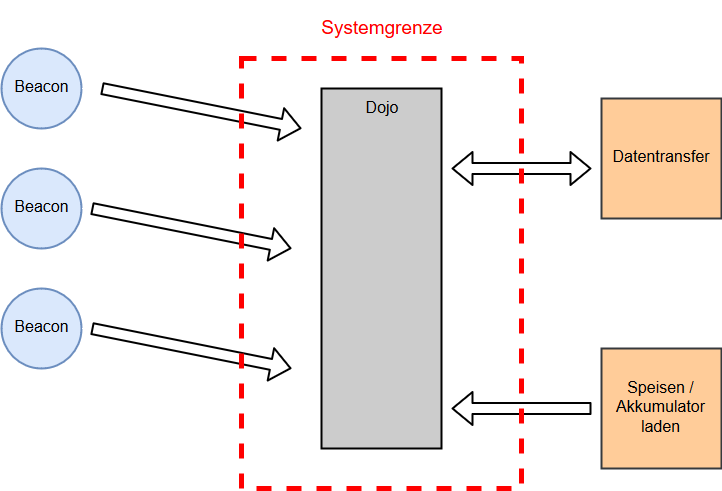
\includegraphics[width=160mm]{data/Loesungskonzept_Systemgrenzen.png}
	\caption{Systemgrenzen des Dojo} %picture caption
	\label{fig:first_layer}
\end{center}
\end{figure}

\subsection{Funktionen}
\subsection{Teilsysteme und ihre Schnittstellen}
\subsection{Alternativer Ansatz}


